\section{Critical Context}

\begin{figure}[h]
 \centering 
 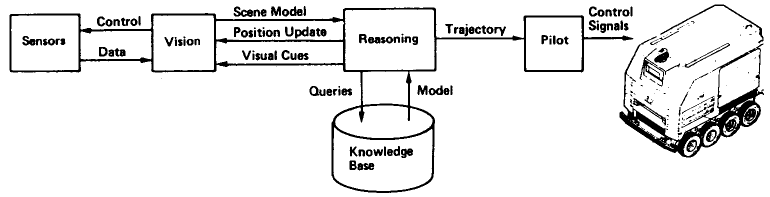
\includegraphics[width=\columnwidth]{figures/ALV-system-configuration.png}
 \caption{The ALV system configuration}
 \label{fig:alv_system_configuration}
\end{figure}

There are several approaches to designing self-driving cars, with respect to acquiring and using sensor data and control systems. At one end of the spectrum is the multi-sensor approach, where cameras, and sensors such as LIDAR and RADAR are used, then all data combined to be processed and generate predictions on steering angle and speed. At the other end is the "camera only" approach, where only images are used to generate a prediction. The former typified by Intel's subsidiary MobileEye, which manufactures the EyeQ5 chip, able of processing dozens of sensor data, including high-resolution cameras, radars, and LiDARs.
citation
https://www.mobileye.com/our-technology/evolution-eyeq-chip/

Then we have NVidia
We need to talk about different approaches such as Intel x NVidia, feature engineering x end-to-end, Elon Musk's problem-will-be-solved-with-computer-vision-alone
In this section we discuss stuff \lipsum[1]

\subsection{Convolutional Neural Networks}

% Tesla
% https://www.tesla.com/en_GB/autopilotAI
Tesla started on MobilEye EyeQ3, moved to NVIDIA DRIVE PX 2 AI, then started developing it's own Tesla-designed processors, currently the HW3 (Hardware 3).

There are a number of tasks related to autonomous-vehicle decision-making. An autonomous vehicle must be able to deal with obstacle detection, scene classification, lane recognition, path planning, motion control, pedestrian detection, traffic signage detection (including traffic lights). 



\subsection{The CNN "End-to-End" approach}



\lipsum[2]

\begin{figure}[h]
 \centering 
 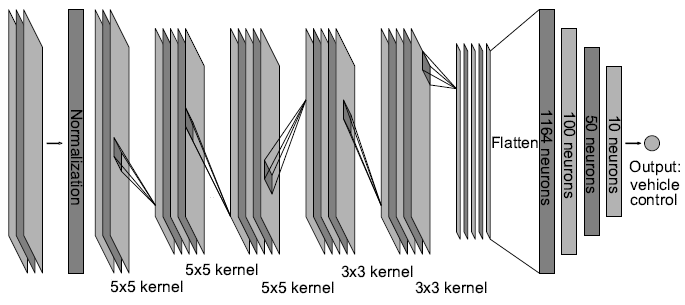
\includegraphics[width=\columnwidth]{figures/nvidia-end-to-end-horizontal.png}
 \caption{NVIDIA End-to-End CNN architecture}
 \label{fig:alv_system_configuration}
\end{figure}

\textbf{TODO} Now what is happening here is, we have an input layer on the left , and we need to all the description as per NVIDIA paper describing the layers and what they are doing.

The NVIDIA CNN architecture we are looking to replicate (Figure \ref{fig:alv_system_configuration}) is a network with about 27 million connections and 250 thousand parameters. At the base are three input 66x200 pixels input planes. Each 

The NVIDIA network was trained with data obtained from about 72 hours of driving. 

\lipsum[2]